\documentclass[12pt]{article}
\usepackage{graphicx} % Required for inserting images
\usepackage[margin=2cm]{geometry}
\usepackage{multicol,amsmath, amssymb}
\usepackage{xcolor}
\usepackage{titlesec}
\usepackage{pgfplots}

\titleformat{\subsection}
{\color{red}\normalfont\Large\bfseries}
{\thesubsection}{1em}{}

\titleformat{\subsubsection}
{\color{blue}\normalfont\large\bfseries}
{\thesubsubsection}{1em}{}

\titlespacing{\subsection}{0pt}{0pt}{0pt} % Adjust the spacing here
\titlespacing{\subsubsection}{0pt}{\baselineskip}{0pt} % Adjust the spacing here
\newcommand{\summation}[2]{\sum\limits^{#1}_{#2}}
\usepackage{fancyhdr}
\usepackage{hyperref} % For hyperlinks

% Define the URL for the footer
\newcommand{\myURL}{https://mohammedbilalns.github.io/Math-Demystified/}

% Set up fancy headers and footers
\pagestyle{fancy}
\fancyhf{} % Clear header and footer
\rfoot{\href{\myURL}{\myURL}} % Set the right part of the footer as a hyperlink

\begin{document}
\begin{center}
    {\LARGE \textbf{Inverse Trigonometric Functions} }
\end{center}

\begin{multicols}{2}
Recall some basic results from class XI
\subsubsection*{Phythagoras' relations}
  $$sin^2 \theta + cos^2 \theta =1 \\
,sec^2 \theta - tan^2 \theta = 1 \\
,cosec^2 \theta - cot^2 \theta =1
$$


\subsubsection*{ Trigonometric Ratios of particular angles}
        \begin{center}
          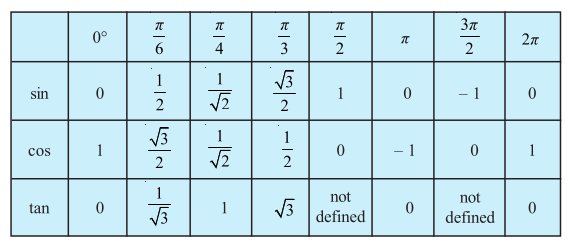
\includegraphics[scale=0.45]{im8.png}
        \end{center}
\subsubsection*{Signs of Trigonometric functions in Quadrants}
            \begin{center}
              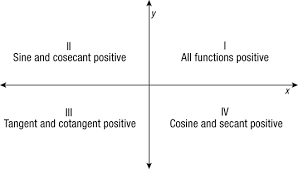
\includegraphics[scale=0.7]{img9.png}
            \end{center}
          
\subsubsection*{Domain and range of trigonometric functions}
              \begin{center}
                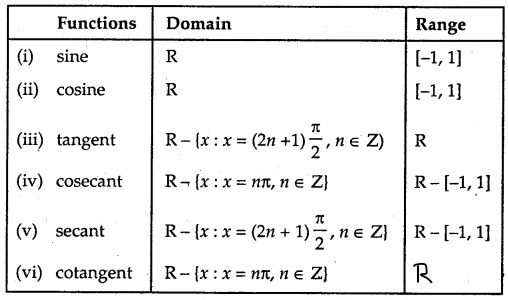
\includegraphics[scale=0.5]{im10.jpg}
              \end{center}

              \subsubsection*{Triganometric Functions of larger angles}
              For an angle $\theta$  and integer n\\
              \begin{align*}
                  sin(n \pi \pm \theta)=sin \theta \\
                  cos(n \pi \pm \theta)=cos \theta \\
                      tan(n \pi \pm \theta)=tan \theta \\
                        cosec(n \pi \pm \theta)=cosec \theta \\
                          sec(n \pi \pm \theta)=sec \theta \\
                            cot(n \pi \pm \theta)=cot \theta \\
              \end{align*}
              ( even multiple of $90^0 + \theta$)
              \begin{align*}
                  sin((2n+1) \frac{\pi}{2} \pm \theta)=cos \theta \\
                  cos((2n+1) \frac{\pi}{2} \pm \theta)=sin \theta \\
                  tan((2n+1) \frac{\pi}{2} \pm \theta)=cot \theta \\
                  cot((2n+1) \frac{\pi}{2} \pm \theta)=tan \theta \\
                  cosec((2n+1) \frac{\pi}{2} \pm \theta)=sec \theta \\
                  sec((2n+1) \frac{\pi}{2} \pm \theta)=cosec \theta \\
              \end{align*}
              (even multiple of $90^0 + \theta$)
              \subsubsection*{Compound Angle Formulas}
              \begin{itemize}
                  \item $sin(x + y) = sin\, x cos y + cos x \,sin y$
              
              \item $sin(x – y) = sin x \,cos y – cos x\, sin y$
              
              \item $cos(x + y) = cos x\, cos y – sin x \,sin y$
              
              \item $cos(x – y) = cos x\, cos y + sin x\, sin y$
              
              \item  $tan ( x + y) =\frac{tan x + tan y}{1 - tan x\, tan y}$
              \item $tan ( x – y) =\frac{tan x – tan y}{1 + tan x\, tan y}$
              \item $cot(x+y)=\frac{cotx \,coty-1}{cot x+cot y}$
              \item  $cot(x-y)=\frac{cotx \,coty+1}{cot x-cot y}$
              
              \end{itemize}
              
              \subsubsection*{ Multiple Angle Formulas}
              \begin{itemize}
                  \item $sin 2x=2 sinx \, cosx=\frac{2tanx}{1+ tan^2 x}$
                  \item $sin 3x = 3 sin x – 4 sin^3 x$
                  \item $cos 2x =cos^2 x - sin^2 x =1- 2sin^2x=2cos^2x-1=\frac{1-tan^2 x}{1+ tan^2 x}$
                  \item  $cos 3x=4 cos^3 x -3 cos x$
                  \item $tan 2x =\frac{2 tan x }{1- tan^2x}$
                  \item $tan 3x=\frac{3 tan x -tan^{3}x}{1-3tan^2(x)}$
                  
              \end{itemize}
    Trigonometric functions are real functions which are not objective and thus its inverse does not exist. In this chapter we study about the restrictions on domains and ranges of trigonometric functions which ensure the existence of their inverse and observe its graphical peculiarities.

\subsection*{Basic Concepts }
In Class XI, we have studied trigonometric functions, which are defined as follows:
\begin{itemize}
    \item sine :$ R \rightarrow [-1,1]$
    \item cos :$ R \rightarrow [-1,1]$
    \item tan :$ R-\{x: x=(2n+1)\frac{\pi}{2}, n \in Z\} \rightarrow R$
    \item cot :$ R-\{x: x=n \pi, n \in Z\} \rightarrow R$
    \item sec :$ R-\{x: x=(2n+1)\frac{\pi}{2}, n \in Z\} \rightarrow R-(-1,1)$
    \item cosec :$ R-\{x: x=n \pi, n \in Z\} \rightarrow R-(-1,1)$
\end{itemize}

These trigonometric functions are onto but not one-one , To define inverse of these trigonometric functions we restrict the domains to \emph{
principal value
branches} and define as follows .


\subsection*{Graphs}
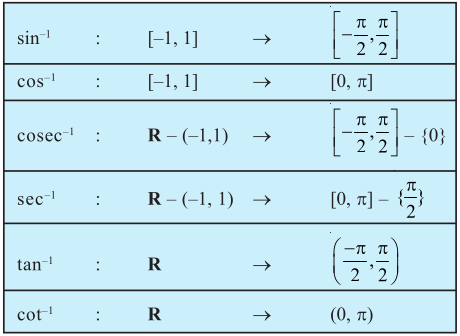
\includegraphics[scale=0.5]{1.png}

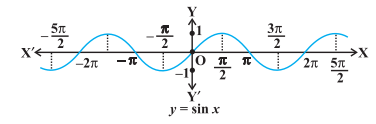
\includegraphics[scale=0.5]{2.png}
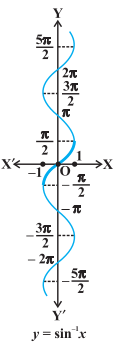
\includegraphics[scale=0.5]{21.png}

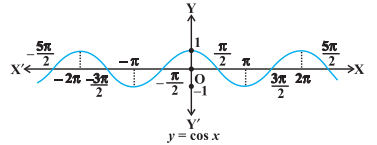
\includegraphics[scale=0.5]{3.png}
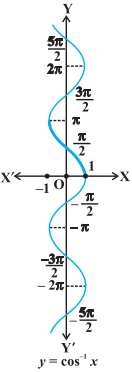
\includegraphics[scale=0.5]{31.png}

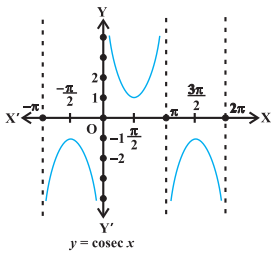
\includegraphics[scale=0.5]{4.png}
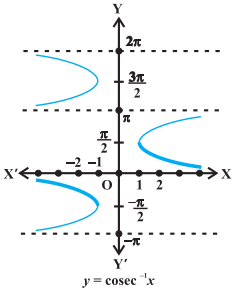
\includegraphics[scale=0.5]{41.png}


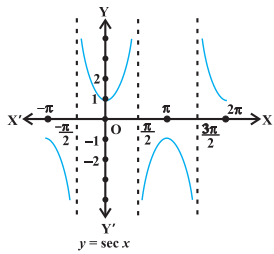
\includegraphics[scale=0.5]{5.png}
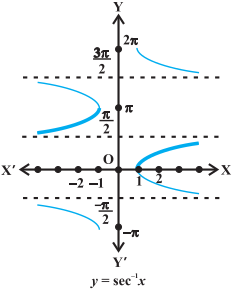
\includegraphics[scale=0.5]{51.png}

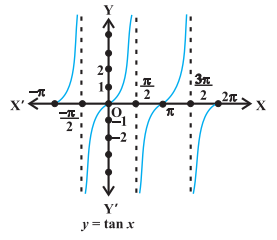
\includegraphics[scale=0.5]{6.png}
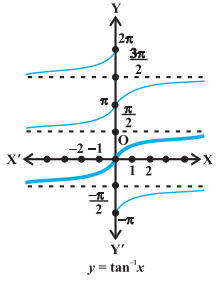
\includegraphics[scale=0.5]{61.png}



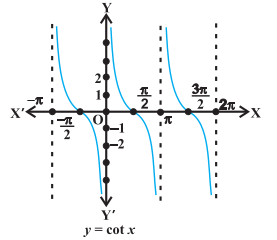
\includegraphics[scale=0.5]{7.png}
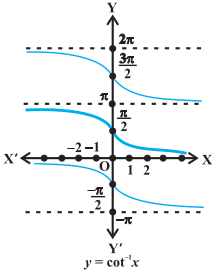
\includegraphics[scale=0.5]{71.png}
\subsubsection*{Note}
\begin{enumerate}
    \item $sin^{-1}x$ should not be confused with $(sin x)^{-1}$. In fact $(sin x)^{-1} =\frac{1}{sin(x)}$ and
similarly for other trigonometric functions.
\item Whenever no branch of an inverse trigonometric functions is mentioned, we
mean the principal value branch of that function.

\item The value of an inverse trigonometric functions which lies in the range of
principal branch is called the \emph{principal value} of that inverse trigonometric
functions.
\end{enumerate}

\subsection*{Properties of Inverse Trigonometric Functions}
\begin{enumerate}
    \item $sin(sin^{-1}x)=x, x \in [-1,1] $
    \item $cos(cos^{-1}x)=x, x \in [-1,1] $
    \item $tan(tan^{-1}x)=x, x \in R $
    \item $cosec(cosec^{-1}x)=x, x \in R-[-1,1] $
    \item $sec(sec^{-1}x)=x, x \in R-[-1,1] $
    \item $cot(cot^{-1}x)=x, x \in R $
    \linebreak
    \item $sin^{-1}(sinx)=x, x \in [\frac{- \pi}{2},\frac{\pi}{2}]$
    \item $cos^{-1}(cosx)=x, x \in [0,\pi]$
    \item $tan^{-1}(tanx)=x, x \in [\frac{- \pi}{2},\frac{\pi}{2}]$
    \item $cosec^{-1}(cosecx)=x, x \in [\frac{- \pi}{2},\frac{\pi}{2}]-\{0\}$
    \item $cos^{-1}(cosx)=x, x \in [0,\pi]-\{\frac{\pi}{2}\}$
    \item $cot^{-1}(cotx)=x, x \in [0,\pi]$
\end{enumerate}

\subsection*{Some Tricks}
\begin{itemize}
  \item For $\sqrt{1-x^2}$ Put $x=sin(\theta)$ or $x=cos(\theta)$
  \item For $\sqrt{1+x^2}$ Put $x=tan(\theta)$ or $x=cot(\theta)$
  \item For $\sqrt{x^2-1}$ Put $x=sec(\theta)$ or $x=cosec(\theta)$

  \item $1-sin(x)=sin^2{\frac{x}{2}}+cos^2{\frac{x}{2}}-2 sin{\frac{x}{2}}cos{\frac{x}{2}}$
   $1+sin(x)=sin^2{\frac{x}{2}}+cos^2{\frac{x}{2}}+2 sin{\frac{x}{2}}cos{\frac{x}{2}}$

\end{itemize}









\end{multicols}

\end{document}